\documentclass[11pt]{article}

% =========================
% Packages
% =========================
\usepackage[margin=0.78in]{geometry}
\usepackage{amsmath,amssymb,amsfonts,mathtools}
\usepackage{booktabs,array,tabularx,longtable,multirow}
\usepackage{enumitem}
\usepackage[most]{tcolorbox}
\usepackage{xcolor}
\usepackage{fancyhdr}
\usepackage{titlesec}
\usepackage{hyperref}
\usepackage{lastpage}
\usepackage{setspace}
\usepackage{tikz}
\usepackage{pgfplots}
\usepackage{needspace}
\usepackage{caption}
\usepackage{multicol}
\usepackage{graphicx}
\usepackage{amsthm}
\usepackage{mathrsfs}
\usepackage{bm}
\usepackage{float}
\usepackage{colortbl}
\usepackage{array}
\usepackage{etoolbox}
\usetikzlibrary{calc,arrows.meta,positioning,decorations.pathreplacing,angles,quotes,intersections,patterns}

\pgfplotsset{compat=1.18}
\setstretch{1.14}
\setlength{\parindent}{0pt}
\setlength{\parskip}{0.45em}
\setlist[itemize]{leftmargin=1.8em}
\setlist[enumerate]{leftmargin=2em}

% =========================
% Colors
% =========================
\definecolor{novelPurple}{RGB}{98,54,255}
\definecolor{novelPurpleDark}{RGB}{72,34,204}
\definecolor{novelPurpleLight}{RGB}{243,239,255}
\definecolor{novelPurpleLine}{RGB}{165,135,255}
\definecolor{npgray}{RGB}{78,78,78}
\definecolor{softgray}{RGB}{246,246,250}
\definecolor{softlav}{RGB}{249,247,255}
\definecolor{greencheck}{RGB}{24,128,88}
\definecolor{warmred}{RGB}{188,54,54}
\definecolor{nporange}{RGB}{223,121,36}
\definecolor{npgreen}{RGB}{67,142,103}
\definecolor{npred}{RGB}{180,54,54}

% =========================
% Hyperref
% =========================
\hypersetup{
    colorlinks=true,
    linkcolor=novelPurpleDark,
    urlcolor=novelPurpleDark,
    citecolor=novelPurpleDark
}

% =========================
% Header / Footer
% =========================
\pagestyle{fancy}
\fancyhf{}
\fancyhead[L]{\textbf{Novel Prep Learning Center}}
\fancyhead[R]{\textbf{AP Calculus AB/BC --- Unit 8}}
\fancyfoot[C]{\textcolor{novelPurpleDark}{\thepage\ /\ \pageref{LastPage}}}
\renewcommand{\headrulewidth}{0.4pt}
\renewcommand{\footrulewidth}{0pt}

% =========================
% Numbering / TOC
% =========================
\setcounter{secnumdepth}{3}
\setcounter{tocdepth}{3}

% =========================
% Section styles
% =========================
\titleformat{\section}
{\Large\bfseries\color{novelPurpleDark}}{\thesection.}{0.6em}{}

\titleformat{\subsection}
{\large\bfseries\color{novelPurple}}{\thesubsection.}{0.6em}{}

\titleformat{\subsubsection}
{\normalsize\bfseries\color{novelPurpleDark}}{\thesubsubsection.}{0.6em}{}

% =========================
% Boxes
% =========================
\tcbset{
  enhanced,
  sharp corners,
  boxrule=1pt
}

\newtcolorbox{theorybox}[1]{
  colback=white,
  colframe=novelPurple,
  colbacktitle=novelPurple,
  coltitle=white,
  title=\textbf{#1},
  fonttitle=\bfseries,
  sharp corners,
  breakable
}

\newtcolorbox{notebox}[1]{
  colback=novelPurpleLight,
  colframe=novelPurple,
  colbacktitle=novelPurple,
  coltitle=white,
  title=\textbf{#1},
  fonttitle=\bfseries,
  sharp corners,
  breakable
}

\newtcolorbox{skillbox}[1]{
  colback=softlav,
  colframe=novelPurpleDark,
  colbacktitle=novelPurpleDark,
  coltitle=white,
  title=\textbf{#1},
  fonttitle=\bfseries,
  sharp corners,
  breakable
}

\newtcolorbox{summarybox}[1]{
  colback=softgray,
  colframe=novelPurpleDark,
  colbacktitle=novelPurpleDark,
  coltitle=white,
  title=\textbf{#1},
  fonttitle=\bfseries,
  sharp corners,
  breakable
}

\newtcolorbox{practicebox}[1]{
  colback=white,
  colframe=novelPurpleLine,
  colbacktitle=novelPurpleLine,
  coltitle=black,
  title=\textbf{#1},
  fonttitle=\bfseries,
  sharp corners,
  breakable
}

\newtcolorbox{homeworkset}[1]{
  colback=white,
  colframe=novelPurpleDark,
  colbacktitle=novelPurpleDark,
  coltitle=white,
  title=\textbf{#1},
  fonttitle=\bfseries,
  sharp corners,
  breakable
}

\newcommand{\hwspace}{\vspace{0.8em}\hrule\vspace{0.8em}}

% =========================
% Commands
% =========================
\newcounter{examplectr}[subsection]
\renewcommand{\theexamplectr}{\thesubsection.\arabic{examplectr}}

\newcommand{\example}[1]{%
\refstepcounter{examplectr}
\Needspace{8\baselineskip}
\noindent{\color{novelPurpleDark}\textbf{Example \theexamplectr.}} \textbf{#1}\par
}

\newcommand{\solution}{\noindent{\textbf{Solution.}}}

\newcommand{\apcheckpoint}[1]{%
\begin{skillbox}{AP Checkpoint}
#1
\end{skillbox}
}

\newcommand{\unitchapter}[1]{%
\newpage
\subsection{#1}
}

\newcommand{\unitsubtopic}[1]{%
\subsubsection{#1}
}

\newcommand{\R}{\mathbb{R}}
\newcommand{\ds}{\displaystyle}

% =========================
% Figure Commands
% =========================

\newcommand{\mvtfigure}{
\begin{center}
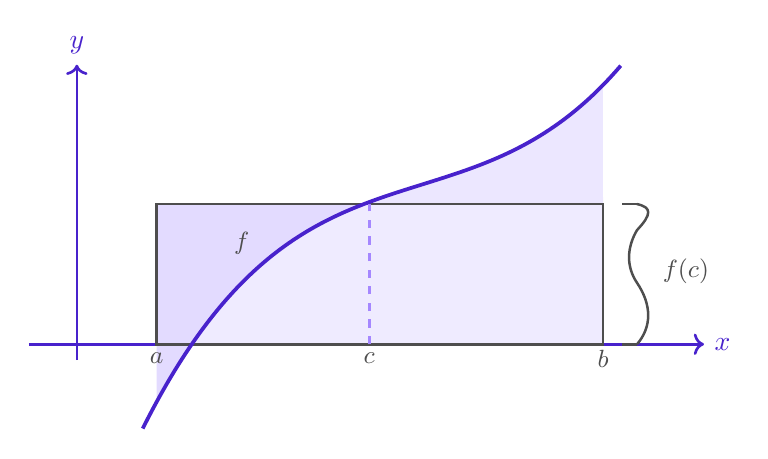
\begin{tikzpicture}[x=1.35cm,y=1.0cm]
    % key values
    \pgfmathsetmacro{\xa}{0.75}
    \pgfmathsetmacro{\xc}{2.75}
    \pgfmathsetmacro{\xb}{4.95}
    \pgfmathsetmacro{\yavg}{1.78}

    % axes
    \draw[novelPurpleDark, line width=0.95pt, ->] (-0.45,0) -- (5.9,0) node[right] {$x$};
    \draw[novelPurpleDark, line width=0.95pt, ->] (0,-0.2) -- (0,3.55) node[above] {$y$};

    % rectangle fill
    \fill[novelPurple!10] (\xa,0) rectangle (\xb,\yavg);

    % top "extra" region above rectangle and under curve (right side)
    \fill[novelPurple!12]
        (\xc,\yavg)
        -- plot[smooth, samples=160, domain=\xc:\xb]
           (\x,{0.11*(\x-2.7)^3 - 0.18*(\x-2.7)^2 + 0.52*(\x-2.7) + 1.78})
        -- (\xb,\yavg) -- cycle;

    % left "missing" region below rectangle and above curve
    \fill[novelPurple!18]
        (\xa,\yavg)
        -- plot[smooth, samples=160, domain=\xa:\xc]
           (\x,{0.11*(\x-2.7)^3 - 0.18*(\x-2.7)^2 + 0.52*(\x-2.7) + 1.78})
        -- (\xc,\yavg) -- cycle;

    % rectangle border
    \draw[npgray, line width=0.95pt] (\xa,0) rectangle (\xb,\yavg);

    % function curve
    \draw[novelPurpleDark, line width=1.35pt, smooth, samples=240, domain=0.62:5.12]
        plot (\x,{0.11*(\x-2.7)^3 - 0.18*(\x-2.7)^2 + 0.52*(\x-2.7) + 1.78});

    % dashed line at c
    \draw[novelPurpleLine, dashed, line width=1pt] (\xc,0) -- (\xc,\yavg);

    % right brace for f(c)
    \draw[npgray, line width=0.9pt]
        (\xb+0.18,0) -- (\xb+0.32,0);
    \draw[npgray, line width=0.9pt]
        (\xb+0.18,\yavg) -- (\xb+0.32,\yavg);
    \draw[npgray, line width=0.9pt]
        (\xb+0.32,0)
        .. controls (\xb+0.46,0.22) and (\xb+0.46,0.50) .. (\xb+0.32,0.78)
        .. controls (\xb+0.22,0.98) and (\xb+0.22,1.22) .. (\xb+0.32,1.45)
        .. controls (\xb+0.46,1.65) and (\xb+0.46,1.74) .. (\xb+0.32,\yavg);

    % labels
    \node[text=npgray] at (1.55,1.28) {\small \(f\)};
    \node[text=npgray] at (\xa,-0.18) {\small \(a\)};
    \node[text=npgray] at (\xc,-0.18) {\small \(c\)};
    \node[text=npgray] at (\xb,-0.18) {\small \(b\)};
    \node[text=npgray] at (\xb+0.78,0.93) {\small \(f(c)\)};
\end{tikzpicture}
\end{center}
}

\newcommand{\velocitysignfigure}{
\begin{center}
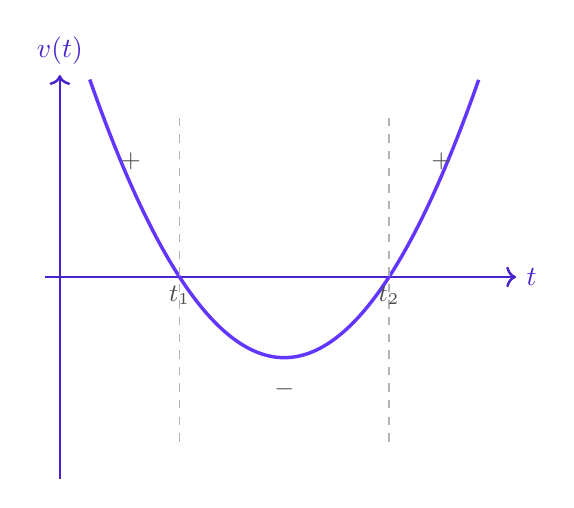
\begin{tikzpicture}[scale=0.95]
\draw[novelPurpleDark, line width=0.9pt, ->] (-0.2,0)--(6.1,0) node[right] {$t$};
\draw[novelPurpleDark, line width=0.9pt, ->] (0,-2.7)--(0,2.7) node[above] {$v(t)$};

\draw[novelPurple, line width=1.25pt, smooth, samples=200, domain=0.4:5.6]
plot (\x,{0.55*(\x-1.6)*(\x-4.4)});
\draw[gray!60, dashed] (1.6,-2.2)--(1.6,2.2);
\draw[gray!60, dashed] (4.4,-2.2)--(4.4,2.2);

\node[text=npgray] at (0.95,1.55) {\small \(+\)};
\node[text=npgray] at (3.0,-1.5) {\small \(-\)};
\node[text=npgray] at (5.1,1.55) {\small \(+\)};
\node[text=npgray] at (1.6,-0.25) {\small \(t_1\)};
\node[text=npgray] at (4.4,-0.25) {\small \(t_2\)};
\end{tikzpicture}
\end{center}
}

\newcommand{\accumulationfigure}{
\begin{center}
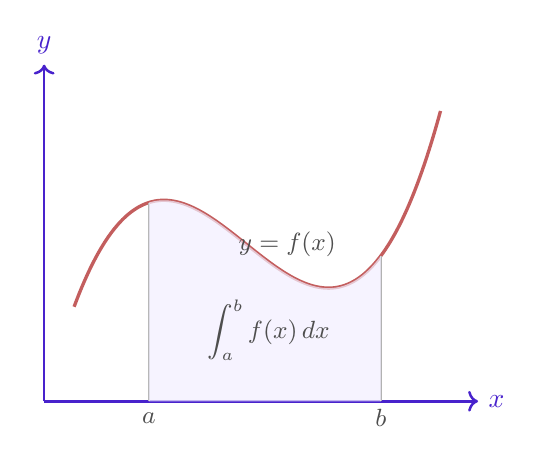
\begin{tikzpicture}[scale=0.95]
\draw[novelPurpleDark, line width=0.9pt, ->] (0,0)--(5.8,0) node[right] {$x$};
\draw[novelPurpleDark, line width=0.9pt, ->] (0,0)--(0,4.5) node[above] {$y$};

\draw[npred!80, line width=1.2pt, smooth, samples=160, domain=0.4:5.3]
plot (\x,{0.22*(\x-2.7)^3 -0.8*(\x-2.7)+2.1});

\draw[gray!60, line width=0.8pt] (1.4,0)--(1.4,{0.22*(1.4-2.7)^3 -0.8*(1.4-2.7)+2.1});
\draw[gray!60, line width=0.8pt] (4.5,0)--(4.5,{0.22*(4.5-2.7)^3 -0.8*(4.5-2.7)+2.1});

\fill[novelPurpleLight, opacity=0.72]
(1.4,0) -- plot[smooth, samples=120, domain=1.4:4.5]
(\x,{0.22*(\x-2.7)^3 -0.8*(\x-2.7)+2.1}) -- (4.5,0) -- cycle;

\node[text=npgray] at (3.25,2.1) {\small \(y=f(x)\)};
\node[text=npgray] at (3.0,0.95) {\small \(\displaystyle \int_a^b f(x)\,dx\)};
\node[text=npgray] at (1.4,-0.22) {\small \(a\)};
\node[text=npgray] at (4.5,-0.22) {\small \(b\)};
\end{tikzpicture}
\end{center}
}

\newcommand{\betweenxfigure}{
\begin{center}
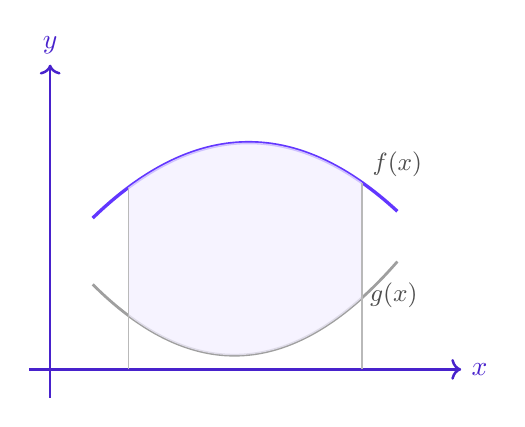
\begin{tikzpicture}[scale=0.9]
\draw[novelPurpleDark, line width=0.9pt, ->] (-0.3,0) -- (5.8,0) node[right] {$x$};
\draw[novelPurpleDark, line width=0.9pt, ->] (0,-0.4) -- (0,4.3) node[above] {$y$};

\draw[novelPurple, line width=1.2pt, smooth, samples=140, domain=0.6:4.9]
plot (\x,{3.2-0.22*(\x-2.8)^2});
\draw[gray!75, line width=1pt, smooth, samples=140, domain=0.6:4.9]
plot (\x,{0.25*(\x-2.6)^2+0.2});

\fill[novelPurpleLight, opacity=0.76]
(1.1,{3.2-0.22*(1.1-2.8)^2})
-- plot[smooth, samples=120, domain=1.1:4.4] (\x,{3.2-0.22*(\x-2.8)^2})
-- plot[smooth, samples=120, domain=4.4:1.1] (\x,{0.25*(\x-2.6)^2+0.2})
-- cycle;

\draw[gray!55] (1.1,0)--(1.1,{3.2-0.22*(1.1-2.8)^2});
\draw[gray!55] (4.4,0)--(4.4,{3.2-0.22*(4.4-2.8)^2});
\node[text=npgray] at (4.9,2.9) {\small \(f(x)\)};
\node[text=npgray] at (4.85,1.05) {\small \(g(x)\)};
\end{tikzpicture}
\end{center}
}

\newcommand{\betweenyfigure}{
\begin{center}
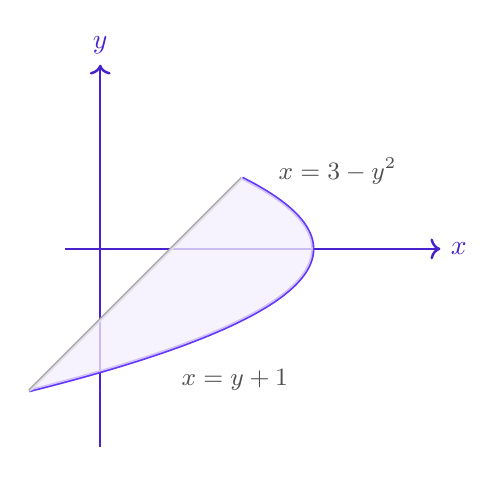
\begin{tikzpicture}[scale=0.9]
\draw[novelPurpleDark, line width=0.9pt, ->] (-0.5,0) -- (4.8,0) node[right] {$x$};
\draw[novelPurpleDark, line width=0.9pt, ->] (0,-2.8) -- (0,2.6) node[above] {$y$};

\draw[novelPurple, line width=1.2pt, smooth, samples=160, domain=-2:1]
plot ({3-\x*\x},{\x});
\draw[gray!70, line width=1.1pt, smooth, samples=160, domain=-2:1]
plot ({\x+1},{\x});

\fill[novelPurpleLight, opacity=0.76]
(1,-2)
-- plot[smooth, samples=120, domain=-2:1] ({3-\x*\x},{\x})
-- plot[smooth, samples=120, domain=1:-2] ({\x+1},{\x})
-- cycle;

\node[text=npgray] at (3.35,1.1) {\small \(x=3-y^2\)};
\node[text=npgray] at (1.9,-1.85) {\small \(x=y+1\)};
\end{tikzpicture}
\end{center}
}

\newcommand{\multiareafigure}{
\begin{center}
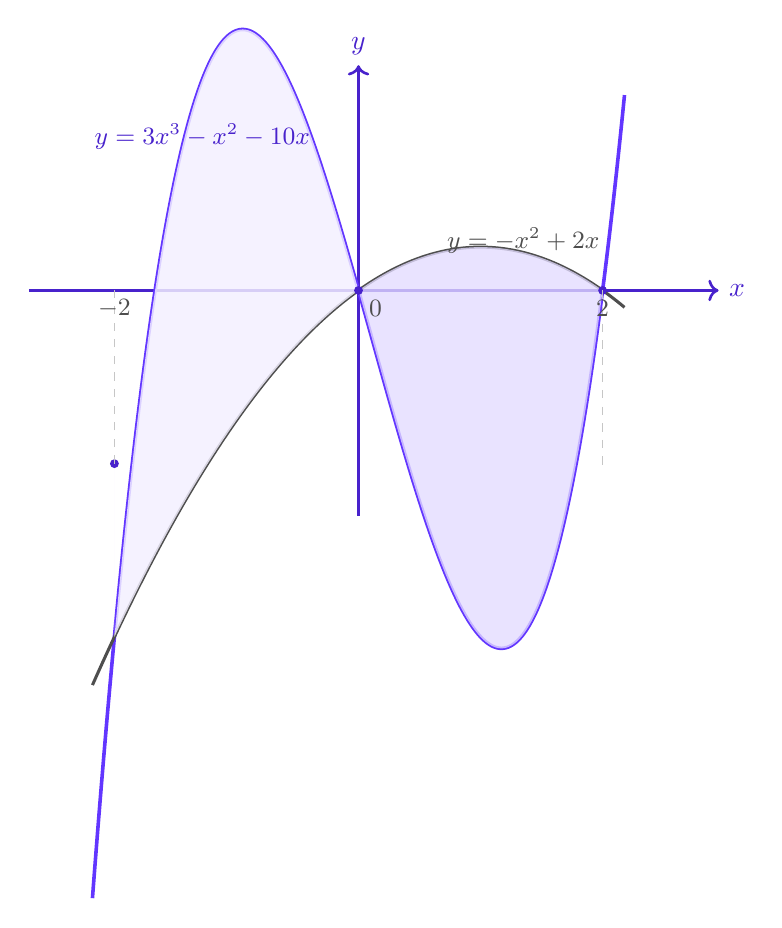
\begin{tikzpicture}[x=1.55cm,y=0.55cm]
    % axes
    \draw[novelPurpleDark, line width=0.95pt, ->] (-2.7,0) -- (2.95,0) node[right] {$x$};
    \draw[novelPurpleDark, line width=0.95pt, ->] (0,-5.2) -- (0,5.2) node[above] {$y$};

    % curves
    \draw[novelPurple, line width=1.3pt, smooth, domain=-2.18:2.18, samples=280]
        plot (\x,{3*(\x)^3 - (\x)^2 - 10*(\x)});
    \draw[npgray, line width=1.1pt, smooth, domain=-2.18:2.18, samples=280]
        plot (\x,{-(\x)^2 + 2*(\x)});

    % left shaded region
    \fill[novelPurpleLight, opacity=0.84]
        (-2,-4)
        -- plot[smooth, domain=-2:0, samples=180]
           (\x,{3*(\x)^3 - (\x)^2 - 10*(\x)})
        -- plot[smooth, domain=0:-2, samples=180]
           (\x,{-(\x)^2 + 2*(\x)})
        -- cycle;

    % right shaded region
    \fill[novelPurple!18, opacity=0.78]
        (0,0)
        -- plot[smooth, domain=0:2, samples=180]
           (\x,{-(\x)^2 + 2*(\x)})
        -- plot[smooth, domain=2:0, samples=180]
           (\x,{3*(\x)^3 - (\x)^2 - 10*(\x)})
        -- cycle;

    % intersection points
    \fill[novelPurpleDark] (-2,-4) circle (1.6pt);
    \fill[novelPurpleDark] (0,0) circle (1.6pt);
    \fill[novelPurpleDark] (2,0) circle (1.6pt);

    % guide lines
    \draw[gray!45, dashed] (-2,-4)--(-2,0);
    \draw[gray!45, dashed] (2,0)--(2,-4.15);

    % labels
    \node[text=novelPurpleDark] at (-1.28,3.55) {\small \(y=3x^3-x^2-10x\)};
    \node[text=npgray] at (1.35,1.15) {\small \(y=-x^2+2x\)};

    % x-axis labels
    \node[text=npgray] at (-2,-0.42) {\small \(-2\)};
    \node[text=npgray] at (0.14,-0.42) {\small \(0\)};
    \node[text=npgray] at (2,-0.42) {\small \(2\)};
\end{tikzpicture}
\end{center}
}

\newcommand{\crosssectionfigure}{
\begin{center}
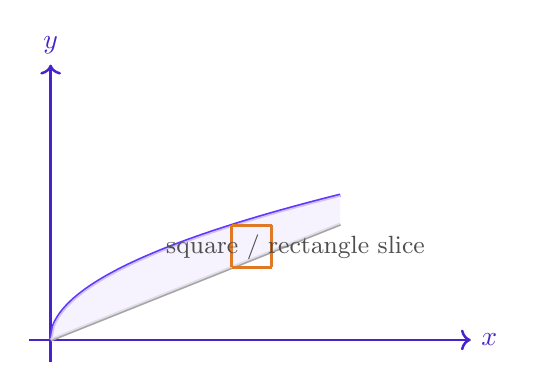
\begin{tikzpicture}[scale=0.92]
\draw[novelPurpleDark, line width=0.9pt, ->] (-0.3,0)--(5.8,0) node[right] {$x$};
\draw[novelPurpleDark, line width=0.9pt, ->] (0,-0.3)--(0,3.8) node[above] {$y$};

\draw[novelPurple, line width=1.2pt, domain=0:4, samples=120] plot (\x,{sqrt(\x)});
\draw[gray!70, line width=1.2pt, domain=0:4, samples=120] plot (\x,{0.4*\x});
\fill[novelPurpleLight, opacity=0.76]
(0,0)--plot[smooth, samples=120, domain=0:4] (\x,{sqrt(\x)})--
plot[smooth, samples=120, domain=4:0] (\x,{0.4*\x})--cycle;

\draw[nporange, line width=1pt] (2.5,{0.4*2.5}) -- (2.5,{sqrt(2.5)});
\draw[nporange, line width=1pt] (2.5,{0.4*2.5}) -- ++(0.55,0);
\draw[nporange, line width=1pt] (2.5,{sqrt(2.5)}) -- ++(0.55,0);
\draw[nporange, line width=1pt] (3.05,{0.4*2.5}) -- (3.05,{sqrt(2.5)});
\node[text=npgray] at (3.38,1.28) {\small square / rectangle slice};
\end{tikzpicture}
\end{center}
}

\newcommand{\trianglecrossfigure}{
\begin{center}
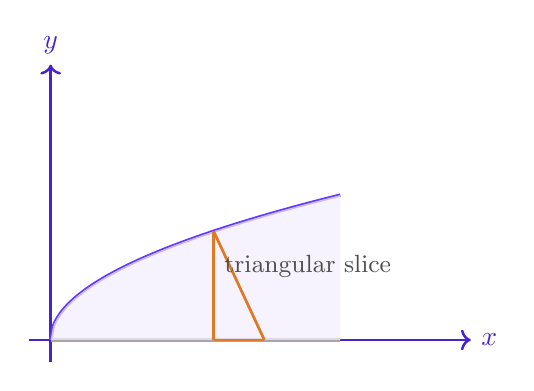
\begin{tikzpicture}[scale=0.92]
\draw[novelPurpleDark, line width=0.9pt, ->] (-0.3,0)--(5.8,0) node[right] {$x$};
\draw[novelPurpleDark, line width=0.9pt, ->] (0,-0.3)--(0,3.8) node[above] {$y$};

\draw[novelPurple, line width=1.2pt, domain=0:4, samples=120] plot (\x,{sqrt(\x)});
\draw[gray!70, line width=1.2pt] (0,0)--(4,0);
\fill[novelPurpleLight, opacity=0.72]
(0,0)--plot[smooth, samples=120, domain=0:4] (\x,{sqrt(\x)})--(4,0)--cycle;

\draw[nporange, line width=1pt] (2.25,0)--(2.25,{sqrt(2.25)});
\draw[nporange, line width=1pt] (2.25,0)--(2.95,0);
\draw[nporange, line width=1pt] (2.25,{sqrt(2.25)})--(2.95,0);
\node[text=npgray] at (3.55,1.02) {\small triangular slice};
\end{tikzpicture}
\end{center}
}

\newcommand{\semicirclecrossfigure}{
\begin{center}
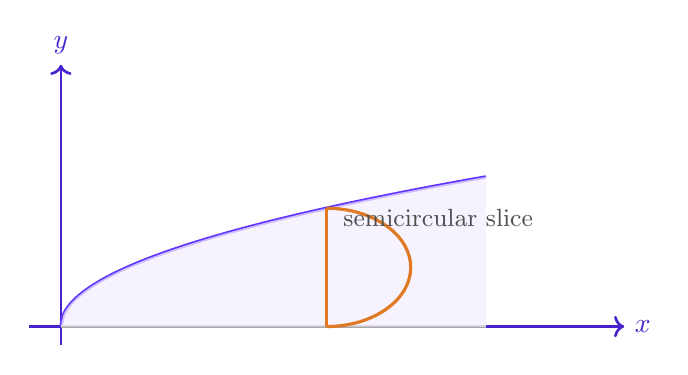
\begin{tikzpicture}[x=1.35cm,y=0.95cm]
    % axes
    \draw[novelPurpleDark, line width=0.95pt, ->] (-0.3,0) -- (5.3,0) node[right] {$x$};
    \draw[novelPurpleDark, line width=0.95pt, ->] (0,-0.25) -- (0,3.5) node[above] {$y$};

    % base region
    \draw[novelPurple, line width=1.25pt, domain=0:4, samples=180]
        plot (\x,{sqrt(\x)});
    \draw[gray!70, line width=1.1pt] (0,0) -- (4,0);

    \fill[novelPurpleLight, opacity=0.74]
        (0,0)
        -- plot[smooth, samples=180, domain=0:4] (\x,{sqrt(\x)})
        -- (4,0) -- cycle;

    % chosen slice
    \pgfmathsetmacro{\xa}{2.5}
    \pgfmathsetmacro{\ya}{sqrt(\xa)}
    \pgfmathsetmacro{\rad}{\ya/2}
    \pgfmathsetmacro{\midy}{\ya/2}

    % diameter
    \draw[nporange, line width=1.15pt] (\xa,0) -- (\xa,\ya);

    % right-opening semicircle
    \draw[nporange, line width=1.15pt]
        (\xa,\ya) arc[start angle=90,end angle=-90,radius=\rad];

    % label
    \node[text=npgray] at (3.55,1.45) {\small semicircular slice};
\end{tikzpicture}
\end{center}
}
\newcommand{\diskfigure}{
\begin{center}
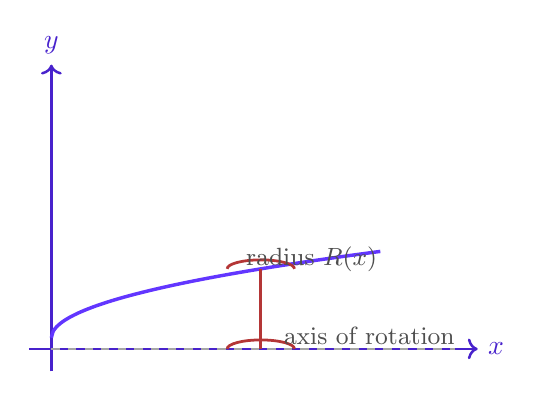
\begin{tikzpicture}[scale=0.95]
\draw[novelPurpleDark, line width=0.9pt, ->] (-0.3,0)--(5.7,0) node[right] {$x$};
\draw[novelPurpleDark, line width=0.9pt, ->] (0,-0.3)--(0,3.8) node[above] {$y$};

\draw[novelPurple, line width=1.25pt, smooth, samples=180, domain=0:4.4]
plot (\x,{0.55*sqrt(\x)+0.15});
\draw[gray!70, dashed, line width=1pt] (0,0)--(5.4,0);

\draw[npred, line width=1pt] (2.8,0) -- (2.8,{0.55*sqrt(2.8)+0.15});
\draw[npred, line width=1pt] (2.35,0) arc[start angle=180,end angle=0,x radius=0.45,y radius=0.12];
\draw[npred, line width=1pt] (2.35,{0.55*sqrt(2.8)+0.15}) arc[start angle=180,end angle=0,x radius=0.45,y radius=0.12];

\node[text=npgray] at (3.48,1.2) {\small radius \(R(x)\)};
\node[text=npgray] at (4.25,0.18) {\small axis of rotation};
\end{tikzpicture}
\end{center}
}

\newcommand{\shifteddiskfigure}{
\begin{center}
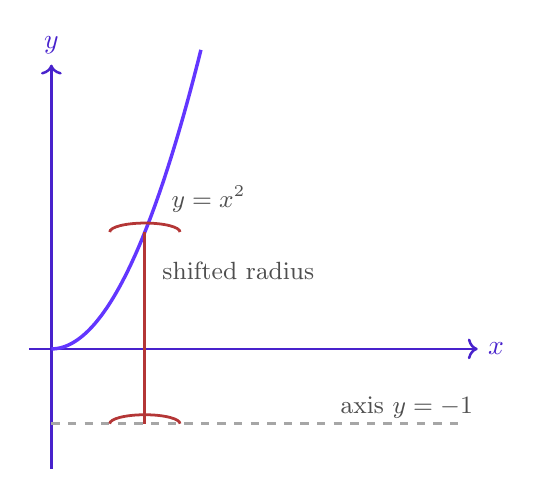
\begin{tikzpicture}[scale=0.95]
\draw[novelPurpleDark, line width=0.9pt, ->] (-0.3,0)--(5.7,0) node[right] {$x$};
\draw[novelPurpleDark, line width=0.9pt, ->] (0,-1.6)--(0,3.8) node[above] {$y$};

\draw[gray!70, dashed, line width=1pt] (0,-1)--(5.45,-1);
\node[text=npgray] at (4.75,-0.78) {\small axis \(y=-1\)};

\draw[novelPurple, line width=1.25pt, smooth, samples=180, domain=0:2]
plot (\x,{(\x)^2});

\draw[npred, line width=1pt] (1.25,-1)--(1.25,{1.25^2});
\draw[npred, line width=1pt] (0.78,-1) arc[start angle=180,end angle=0,x radius=0.47,y radius=0.12];
\draw[npred, line width=1pt] (0.78,{1.25^2}) arc[start angle=180,end angle=0,x radius=0.47,y radius=0.12];

\node[text=npgray] at (2.1,2.0) {\small \(y=x^2\)};
\node[text=npgray] at (2.5,1.05) {\small shifted radius};
\end{tikzpicture}
\end{center}
}

\newcommand{\washerfigure}{
\begin{center}
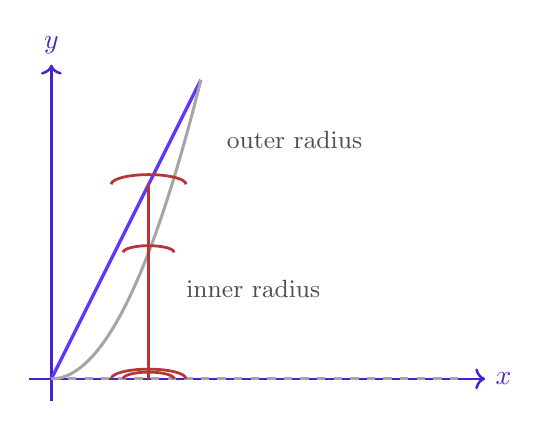
\begin{tikzpicture}[scale=0.95]
\draw[novelPurpleDark, line width=0.9pt, ->] (-0.3,0)--(5.8,0) node[right] {$x$};
\draw[novelPurpleDark, line width=0.9pt, ->] (0,-0.3)--(0,4.2) node[above] {$y$};

\draw[gray!70, dashed, line width=1pt] (0,0)--(5.5,0);
\draw[novelPurple, line width=1.2pt, smooth, samples=140, domain=0:2]
plot (\x,{2*\x});
\draw[gray!70, line width=1.1pt, smooth, samples=140, domain=0:2]
plot (\x,{(\x)^2});

\draw[npred, line width=1pt] (1.3,0)--(1.3,{2*1.3});
\draw[npred, line width=1pt] (1.3,0)--(1.3,{1.3^2});
\draw[npred, line width=1pt] (0.8,0) arc[start angle=180,end angle=0,x radius=0.5,y radius=0.13];
\draw[npred, line width=1pt] (0.96,0) arc[start angle=180,end angle=0,x radius=0.34,y radius=0.09];
\draw[npred, line width=1pt] (0.8,{2*1.3}) arc[start angle=180,end angle=0,x radius=0.5,y radius=0.13];
\draw[npred, line width=1pt] (0.96,{1.3^2}) arc[start angle=180,end angle=0,x radius=0.34,y radius=0.09];

\node[text=npgray] at (3.25,3.2) {\small outer radius};
\node[text=npgray] at (2.7,1.2) {\small inner radius};
\end{tikzpicture}
\end{center}
}

\newcommand{\shiftedwasherfigure}{
\begin{center}
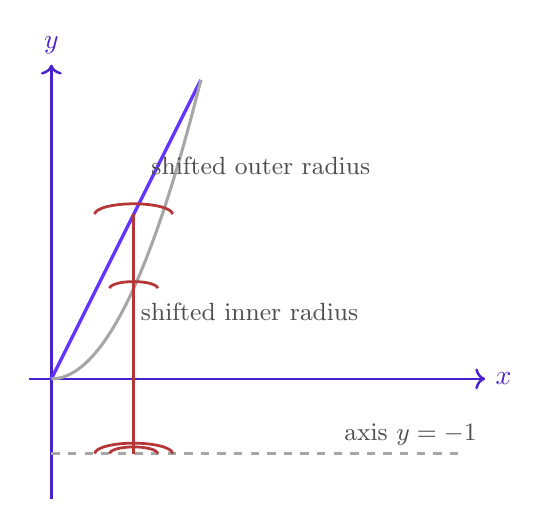
\begin{tikzpicture}[scale=0.95]
\draw[novelPurpleDark, line width=0.9pt, ->] (-0.3,0)--(5.8,0) node[right] {$x$};
\draw[novelPurpleDark, line width=0.9pt, ->] (0,-1.6)--(0,4.2) node[above] {$y$};

\draw[gray!70, dashed, line width=1pt] (0,-1)--(5.5,-1);
\node[text=npgray] at (4.8,-0.75) {\small axis \(y=-1\)};

\draw[novelPurple, line width=1.2pt, smooth, samples=140, domain=0:2]
plot (\x,{2*\x});
\draw[gray!70, line width=1.1pt, smooth, samples=140, domain=0:2]
plot (\x,{(\x)^2});

\draw[npred, line width=1pt] (1.1,-1)--(1.1,{2*1.1});
\draw[npred, line width=1pt] (1.1,-1)--(1.1,{1.1^2});
\draw[npred, line width=1pt] (0.58,-1) arc[start angle=180,end angle=0,x radius=0.52,y radius=0.14];
\draw[npred, line width=1pt] (0.78,-1) arc[start angle=180,end angle=0,x radius=0.32,y radius=0.09];
\draw[npred, line width=1pt] (0.58,{2*1.1}) arc[start angle=180,end angle=0,x radius=0.52,y radius=0.14];
\draw[npred, line width=1pt] (0.78,{1.1^2}) arc[start angle=180,end angle=0,x radius=0.32,y radius=0.09];

\node[text=npgray] at (2.8,2.85) {\small shifted outer radius};
\node[text=npgray] at (2.65,0.9) {\small shifted inner radius};
\end{tikzpicture}
\end{center}
}

% =========================================================
\begin{document}

% =========================================================
% Cover Page
% =========================================================
\begin{titlepage}
\centering
\vspace*{2.0cm}

{\fontsize{28}{32}\selectfont\bfseries\color{novelPurpleDark} AP Calculus AB \& BC\par}
\vspace{0.35cm}
{\fontsize{28}{32}\selectfont\bfseries\color{novelPurpleDark} Unit 8: Applications of Integration\par}

\vspace{0.7cm}


\vspace{1cm}

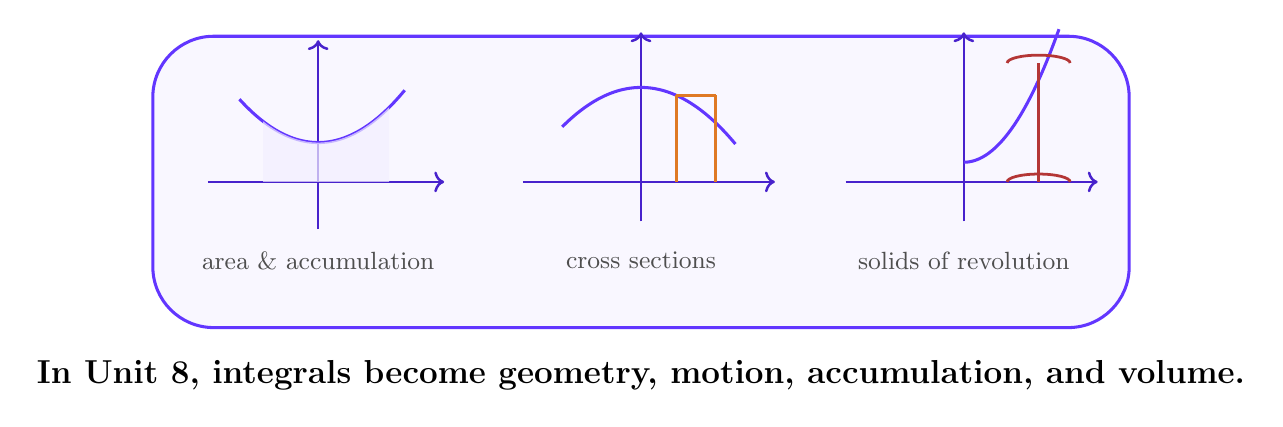
\begin{tikzpicture}[scale=1]
\fill[softlav,rounded corners=22pt] (-6.2,-1.85) rectangle (6.2,1.85);
\draw[novelPurple, line width=1.1pt, rounded corners=22pt] (-6.2,-1.85) rectangle (6.2,1.85);

\begin{scope}[shift={(-4.1,0)}]
\draw[novelPurpleDark, line width=0.9pt, ->] (-1.4,0)--(1.6,0);
\draw[novelPurpleDark, line width=0.9pt, ->] (0,-0.6)--(0,1.8);
\draw[novelPurple, line width=1.1pt, smooth, samples=120, domain=-1:1.1]
plot (\x,{0.55*\x*\x+0.5});
\fill[novelPurpleLight, opacity=0.7] (-0.7,0) -- plot[smooth, samples=80, domain=-0.7:0.9] (\x,{0.55*\x*\x+0.5}) -- (0.9,0)--cycle;
\node[text=npgray] at (0,-1.0) {\small area \& accumulation};
\end{scope}

\begin{scope}[shift={(0,0)}]
\draw[novelPurpleDark, line width=0.9pt, ->] (-1.5,0)--(1.7,0);
\draw[novelPurpleDark, line width=0.9pt, ->] (0,-0.5)--(0,1.9);
\draw[novelPurple, line width=1.1pt, domain=-1:1.2, samples=120] plot (\x,{1.2-0.5*\x*\x});
\draw[nporange, line width=1pt] (0.45,0)--(0.45,{1.2-0.5*(0.45)^2});
\draw[nporange, line width=1pt] (0.95,0)--(0.95,{1.2-0.5*(0.45)^2});
\draw[nporange, line width=1pt] (0.45,{1.2-0.5*(0.45)^2})--(0.95,{1.2-0.5*(0.45)^2});
\node[text=npgray] at (0,-1.0) {\small cross sections};
\end{scope}

\begin{scope}[shift={(4.1,0)}]
\draw[novelPurpleDark, line width=0.9pt, ->] (-1.5,0)--(1.7,0);
\draw[novelPurpleDark, line width=0.9pt, ->] (0,-0.5)--(0,1.9);
\draw[novelPurple, line width=1.1pt, domain=0:1.1, samples=120] plot ({1.1*\x},{1.4*\x*\x+0.25});
\draw[npred, line width=1pt] (0.95,0)--(0.95,1.51);
\draw[npred, line width=1pt] (0.55,0) arc[start angle=180,end angle=0,x radius=0.4,y radius=0.1];
\draw[npred, line width=1pt] (0.55,1.51) arc[start angle=180,end angle=0,x radius=0.4,y radius=0.1];
\node[text=npgray] at (0,-1.0) {\small solids of revolution};
\end{scope}

\node[align=center] at (0,-2.45) {\large\bfseries In Unit 8, integrals become geometry, motion, accumulation, and volume.};
\end{tikzpicture}

\vfill

\begin{minipage}{0.84\textwidth}
\begin{notebox}{Second Optimization Goals}
\begin{itemize}
    \item Keep the complete Unit 8 structure from the original handout.
    \item Preserve the original theorem / example flow as much as possible.
    \item Rebuild every major diagram in cleaner, more accurate TikZ form.
    \item Make each theorem section immediately readable with a matching picture when helpful.
\end{itemize}
\end{notebox}
\end{minipage}

\vfill

{\large\textbf{Novel Prep Learning Center}}\\[0.25em]
{\large J.Z}

\end{titlepage}

\tableofcontents
\newpage

% =========================================================
\setcounter{section}{7}
\section{Applications of Integration}

\begin{theorybox}{Big Idea}
An integral is not only an antiderivative tool. In this unit, definite integrals describe:
\begin{itemize}
    \item average values,
    \item displacement and total distance,
    \item accumulation of changing quantities,
    \item area between curves,
    \item volumes by slicing,
    \item and volumes of solids of revolution.
\end{itemize}
\end{theorybox}

\begin{notebox}{Teaching Philosophy for This Unit}
Students should stop thinking of \(\int\) as “just undoing a derivative.” In Unit 8, the integral becomes a geometric and physical language:
\[
\text{rate} \longrightarrow \text{accumulation},
\qquad
\text{slice} \longrightarrow \text{total volume},
\qquad
\text{height difference} \longrightarrow \text{area}.
\]
\end{notebox}

\apcheckpoint{
When a problem involves a changing rate, a continuously varying cross section, or a region built from infinitely many slices, a definite integral is usually the correct model.
}

% =========================================================
\unitchapter{Average Value of a Function on an Interval}

\unitsubtopic{The Mean Value Theorem for Integrals}

\begin{theorybox}{Theorem 8.1.1 --- Mean Value Theorem for Integrals}
If \(f\) is continuous on the closed interval \([a,b]\), then there exists a number \(c\in[a,b]\) such that
\[
\int_a^b f(x)\,dx = f(c)(b-a).
\]
Equivalently,
\[
f(c)=\frac{1}{b-a}\int_a^b f(x)\,dx.
\]
\end{theorybox}

\mvtfigure

\begin{summarybox}{What the Theorem Says Geometrically}
The rectangle with width \(b-a\) and height \(f(c)\) has the same area as the area under \(f(x)\) from \(a\) to \(b\).
\end{summarybox}
\newpage
\unitsubtopic{Average Value of a Function}

\begin{theorybox}{Theorem 8.1.2 --- Average Value of a Function on an Interval}
If \(f\) is integrable on the closed interval \([a,b]\), then the average value of \(f\) on the interval is
\[
f_{\mathrm{avg}}=\frac{1}{b-a}\int_a^b f(x)\,dx.
\]
\end{theorybox}

\mvtfigure

\example{Finding the average value of a function}
Find the average value of
\[
f(x)=3x^2-2x
\]
on the interval \([1,4]\).

\solution
\[
f_{\mathrm{avg}}=\frac{1}{4-1}\int_1^4 (3x^2-2x)\,dx
= \frac13\left[x^3-x^2\right]_1^4.
\]
Evaluate:
\[
\left[x^3-x^2\right]_1^4=(64-16)-(1-1)=48.
\]
So
\[
f_{\mathrm{avg}}=\frac{48}{3}=16.
\]

\example{Average velocity as an average value}
Show that the average velocity of a car over the time interval \([t_1,t_2]\) is the same as the average value of its velocity function over that interval.

\solution
If \(s(t)\) is displacement, then average velocity by definition is
\[
\frac{s(t_2)-s(t_1)}{t_2-t_1}.
\]
The average value of the velocity function \(v(t)=s'(t)\) is
\[
\frac{1}{t_2-t_1}\int_{t_1}^{t_2}v(t)\,dt
=
\frac{1}{t_2-t_1}\int_{t_1}^{t_2}s'(t)\,dt.
\]
By the Net Change Theorem,
\[
\int_{t_1}^{t_2}s'(t)\,dt=s(t_2)-s(t_1).
\]
Therefore
\[
\frac{1}{t_2-t_1}\int_{t_1}^{t_2}v(t)\,dt
=
\frac{s(t_2)-s(t_1)}{t_2-t_1}.
\]

% =========================================================
\unitchapter{Position, Velocity, and Acceleration}

\unitsubtopic{Integrating Velocity to Find Position}

\begin{theorybox}{Theorem 8.2.1 --- Integral of Velocity}
If \(v(t)\) is the velocity of an object, then the position function is
\[
s(t)=\int v(t)\,dt + C,
\]
where \(C\) is determined by the initial position.
\end{theorybox}

\begin{theorybox}{Theorem 8.2.2 --- Displacement}
The displacement of an object over a time interval \([a,b]\) is
\[
\Delta s=s(b)-s(a)=\int_a^b v(t)\,dt.
\]
\end{theorybox}

\begin{theorybox}{Theorem 8.2.3 --- Distance Traveled}
The total distance traveled over \([a,b]\) is
\[
\int_a^b |v(t)|\,dt.
\]
Absolute value is necessary because distance ignores direction.
\end{theorybox}

\velocitysignfigure

\example{Position from velocity}
Suppose an object has velocity
\[
v(t)=2t+5
\]
with initial position \(s(0)=10\). Find the position function \(s(t)\).

\solution
Integrate velocity:
\[
s(t)=\int (2t+5)\,dt + C = t^2+5t+C.
\]
Since \(s(0)=10\), we have \(C=10\). Thus
\[
s(t)=t^2+5t+10.
\]

\example{Displacement and distance traveled}
Given the velocity function
\[
v(t)=3t-2
\]
on the interval \([1,4]\), find the displacement and distance traveled.

\solution
Displacement:
\[
\int_1^4 (3t-2)\,dt
=
\left[\frac32 t^2-2t\right]_1^4
=
(24-8)-\left(\frac32-2\right)
=
16+\frac12
=
\frac{33}{2}.
\]
Since \(v(t)=3t-2>0\) on \(1\le t\le 4\), the velocity never changes sign, so
\[
\int_1^4 |3t-2|\,dt=\frac{33}{2}.
\]
\newpage
\unitsubtopic{Integrating Acceleration to Find Velocity}

\begin{theorybox}{Theorem 8.2.4 --- Integrating Acceleration to Find Velocity}
If \(a(t)\) is the acceleration of an object, then its velocity is
\[
v(t)=\int a(t)\,dt + C,
\]
where \(C\) is determined by the initial velocity.
\end{theorybox}

\velocitysignfigure

\example{From acceleration to position}
A particle moves along the \(y\)-axis with acceleration
\[
a(t)=2.
\]
Its velocity at \(t=2\) is \(5\) cm/sec, and its position at \(t=2\) is \(10\) cm. Find its position at \(t=6\).

\solution
First find velocity:
\[
v(t)=\int 2\,dt = 2t+C.
\]
Use \(v(2)=5\):
\[
5=4+C \quad\Rightarrow\quad C=1.
\]
So
\[
v(t)=2t+1.
\]
Now find position:
\[
x(t)=\int (2t+1)\,dt=t^2+t+C.
\]
Use \(x(2)=10\):
\[
10=4+2+C \quad\Rightarrow\quad C=4.
\]
Thus
\[
x(t)=t^2+t+4.
\]
At \(t=6\),
\[
x(6)=36+6+4=46.
\]
So the position is
\[
\boxed{46\text{ cm}}.
\]

% =========================================================
\unitchapter{Using Accumulation Functions and Definite Integrals}

\unitsubtopic{Accumulation Functions}

\begin{theorybox}{Definition 8.3.1 --- Accumulation Functions}
A definite integral
\[
\int_a^b f(x)\,dx
\]
represents the accumulation of the quantity described by \(f(x)\) over the interval \([a,b]\).
\end{theorybox}

\accumulationfigure

\begin{notebox}{Accumulation Function: Steps to Follow}
\begin{enumerate}
    \item Identify the rate-of-change function.
    \item Set up the definite integral for total change.
    \item Evaluate the integral.
    \item Use any initial condition if the problem asks for a total quantity rather than just a net change.
\end{enumerate}
\end{notebox}

\example{Rate of oil consumption}
The rate of consumption of oil in the United States during the 1980s is modeled by
\[
R(t)=27.08e^{t/25}
\]
billion barrels per year, where \(t\) is the number of years after January 1, 1980. Find the total oil consumption during the 1980s.

\solution
The total oil consumption is
\[
\int_0^{10} 27.08e^{t/25}\,dt.
\]
Compute:
\[
\int 27.08e^{t/25}\,dt = 27.08\cdot 25\, e^{t/25}=677e^{t/25}.
\]
So
\[
\int_0^{10}27.08e^{t/25}\,dt
=
677\left(e^{10/25}-1\right)
=
677\left(e^{0.4}-1\right).
\]
Numerically,
\[
677(e^{0.4}-1)\approx 332.965.
\]
Thus the total consumption is approximately
\[
\boxed{332.965\text{ billion barrels}}.
\]

\example{Population growth from a rate model}
The population of a city is modeled by
\[
P(t)=5000e^{0.03t},
\]
where \(t\) is the number of years since 2000. Find the total accumulated value from 2000 to 2020.

\solution
We compute
\[
\int_0^{20} 5000e^{0.03t}\,dt.
\]
An antiderivative is
\[
\frac{5000}{0.03}e^{0.03t}.
\]
So
\[
\int_0^{20}5000e^{0.03t}\,dt
=
\frac{5000}{0.03}\left(e^{0.6}-1\right).
\]
Numerically,
\[
\frac{5000}{0.03}(e^{0.6}-1)\approx 136800.
\]

\example{Mosquito population on Tropical Island}
For \(0\le t\le 31\), the rate of change of the number of mosquitoes on Tropical Island is modeled by
\[
R(t)=5\sqrt{t}\cos\left(\frac{t}{5}\right)
\]
mosquitoes per day. There are \(1000\) mosquitoes at \(t=0\).

\begin{enumerate}[label=\textbf{(\alph*)}]
\item Show that the number of mosquitoes is increasing at \(t=6\).
\item At \(t=6\), is the number of mosquitoes increasing at an increasing rate or at a decreasing rate?
\item According to the model, how many mosquitoes are on the island at \(t=31\)?
\end{enumerate}

\solution
\textbf{(a)} Since \(R(t)\) is the rate of change of the mosquito population, the population is increasing when \(R(t)>0\).
\[
R(6)=5\sqrt6\cos\left(\frac65\right).
\]
Because \(\cos(1.2)>0\), we get \(R(6)>0\).

\textbf{(b)} Differentiate:
\[
R'(t)=\frac{5}{2\sqrt t}\cos\left(\frac{t}{5}\right)-\sqrt t\sin\left(\frac{t}{5}\right).
\]
Evaluating numerically at \(t=6\) gives \(R'(6)<0\). So the number of mosquitoes is increasing at a decreasing rate.

\textbf{(c)} Population at \(t=31\):
\[
N(31)=1000+\int_0^{31}5\sqrt t\cos\left(\frac{t}{5}\right)\,dt.
\]
Numerically,
\[
\int_0^{31}5\sqrt t\cos\left(\frac{t}{5}\right)\,dt\approx 139.51.
\]
Thus
\[
N(31)\approx 1000+139.51\approx 1140.
\]

% =========================================================
\unitchapter{Finding the Area Between Curves (Expressed as Functions of \(x\))}

\begin{theorybox}{Theorem 8.4.1 --- Area of a Region Between Two Curves}
If \(f\) and \(g\) are continuous on \([a,b]\) and \(g(x)\le f(x)\) for all \(x\in[a,b]\), then the area of the region bounded by the graphs of \(f\) and \(g\) and the vertical lines \(x=a\) and \(x=b\) is
\[
A=\int_a^b [f(x)-g(x)]\,dx.
\]
\end{theorybox}

\betweenxfigure

\example{Area between two curves}
Find the area of the region bounded by
\[
y=x^2+2,\qquad y=-x,\qquad x=0,\qquad x=1.
\]

\solution
Top minus bottom:
\[
A=\int_0^1 \big[(x^2+2)-(-x)\big]\,dx
=\int_0^1 (x^2+x+2)\,dx.
\]
Integrate:
\[
A=\left[\frac{x^3}{3}+\frac{x^2}{2}+2x\right]_0^1
=
\frac13+\frac12+2
=
\frac{17}{6}.
\]

\example{A region lying between two intersecting graphs}
Find the area of the region bounded by
\[
f(x)=e^x
\qquad\text{and}\qquad
g(x)=x+2.
\]

\solution
We solve
\[
e^x=x+2
\]
numerically. The two intersections are approximately
\[
x\approx -1.8414
\quad\text{and}\quad
x\approx 1.1462.
\]
On this interval, \(g(x)\ge f(x)\), so
\[
A=\int_{-1.8414}^{1.1462}\big[(x+2)-e^x\big]\,dx.
\]
An antiderivative is
\[
\frac{x^2}{2}+2x-e^x.
\]
Thus
\[
A\approx 1.532.
\]

\example{Area between \(\ln(x+3)\) and a polynomial}
Let
\[
f(x)=\ln(x+3),\qquad g(x)=x^4+2x^3.
\]
The graphs intersect at \(x=-2\) and at \(x=B\), where \(B>0\). The positive intersection is approximately
\[
B\approx 0.782.
\]
Find the area enclosed by the graphs.

\solution
The required area is
\[
A=\int_{-2}^{0.782}\left[\ln(x+3)-(x^4+2x^3)\right]\,dx.
\]
Using numerical evaluation,
\[
A\approx 3.604.
\]

% =========================================================
\unitchapter{Finding the Area Between Curves (Expressed as Functions of \(y\))}

\begin{theorybox}{Theorem 8.5.1 --- Area of a Region Between Two Curves in Terms of \(y\)}
When a region is more naturally described using horizontal slices, the area is
\[
A=\int_c^d [x_{\text{right}}(y)-x_{\text{left}}(y)]\,dy.
\]
\end{theorybox}

\betweenyfigure

\begin{notebox}{Common Pitfalls}
\begin{itemize}
    \item Switching left and right functions.
    \item Using \(x\)-bounds instead of \(y\)-bounds.
    \item Forgetting to split the integral if the “right minus left” order changes.
\end{itemize}
\end{notebox}

\example{Horizontal representative rectangles}
Find the area of the region bounded by
\[
x=3-y^2
\qquad\text{and}\qquad
x=y+1.
\]

\solution
First solve intersections:
\[
3-y^2=y+1
\quad\Longrightarrow\quad
y^2+y-2=0
\quad\Longrightarrow\quad
y=-2,\;1.
\]
For \(-2\le y\le 1\), the right-hand curve is \(x=3-y^2\) and the left-hand curve is \(x=y+1\). So
\[
A=\int_{-2}^{1}\big[(3-y^2)-(y+1)\big]\,dy
=\int_{-2}^{1}(-y^2-y+2)\,dy.
\]
Integrate:
\[
A=\left[-\frac{y^3}{3}-\frac{y^2}{2}+2y\right]_{-2}^{1}
=\frac{9}{2}.
\]

\example{Area between curves in terms of \(y\)}
Find the area of the region bounded by
\[
x=y^2
\qquad\text{and}\qquad
x=4.
\]

\solution
Intersections occur when
\[
y^2=4 \quad\Longrightarrow\quad y=\pm 2.
\]
So
\[
A=\int_{-2}^{2}(4-y^2)\,dy
=\left[4y-\frac{y^3}{3}\right]_{-2}^{2}
=16-\frac{16}{3}
=\frac{32}{3}.
\]

% =========================================================
\unitchapter{Finding the Area Between Curves (Intersect at More Than Two Points)}

\begin{theorybox}{Key Idea}
If the “top minus bottom” order changes, split the region into separate integrals and add absolute areas.
\end{theorybox}

\multiareafigure

\example{Curves that intersect at more than two points}
Find the area of the region between
\[
f(x)=3x^3-x^2-10x
\qquad\text{and}\qquad
g(x)=-x^2+2x.
\]

\solution
Set \(f(x)=g(x)\):
\[
3x^3-x^2-10x=-x^2+2x
\quad\Longrightarrow\quad
3x^3-12x=0
\quad\Longrightarrow\quad
3x(x^2-4)=0.
\]
So intersections are
\[
x=-2,\;0,\;2.
\]
Now
\[
f(x)-g(x)=3x^3-12x.
\]
On \([-2,0]\), \(f(x)\ge g(x)\), and on \([0,2]\), \(g(x)\ge f(x)\). Therefore
\[
A=\int_{-2}^{0}(3x^3-12x)\,dx+\int_0^2(-3x^3+12x)\,dx.
\]
This evaluates to
\[
A=24.
\]

\example{Writing an area as a sum of integrals}
The figure shows the graphs of \(y=|x|\) and \(y=3+2x-x^2\) for \(-1\le x\le 3\). The \(x\)-coordinates of the points of intersection are \(x_1\) and \(x_2\), where \(x_1<x_2\). Write a sum of integrals that represents the shaded regions.

\solution
Because \(|x|\) changes rule at \(x=0\), one valid setup is
\[
\int_{-1}^{x_1}(x^2-3x-3)\,dx
+\int_{x_1}^{0}(-x^2+3x+3)\,dx
+\int_{0}^{x_2}(-x^2+x+3)\,dx
+\int_{x_2}^{3}(x^2-x-3)\,dx.
\]

% =========================================================
\unitchapter{Volumes with Cross Sections: Squares and Rectangles}

\begin{theorybox}{Theorem 8.7.1 --- Volumes of Solids with Known Cross Sections}
If the cross-sectional area is \(A(x)\) perpendicular to the \(x\)-axis, then
\[
V=\int_a^b A(x)\,dx.
\]
If the cross-sectional area is \(A(y)\) perpendicular to the \(y\)-axis, then
\[
V=\int_c^d A(y)\,dy.
\]
\end{theorybox}

\crosssectionfigure

\unitsubtopic{Rectangular Cross Sections}

\begin{theorybox}{Theorem 8.7.2 --- Rectangular Cross Sections}
If each cross section is a rectangle with base \(b(x)\) and height \(h(x)\), then
\[
A(x)=b(x)h(x),
\qquad
V=\int_a^b b(x)h(x)\,dx.
\]
\end{theorybox}

\crosssectionfigure

\example{Rectangular cross sections}
Suppose the base region is bounded by
\[
x=y^3
\qquad\text{and}\qquad
x=2,
\]
for \(0\le y\le \sqrt[3]{2}\). Each cross section perpendicular to the \(y\)-axis is a rectangle whose height is \(6\) times its base. Find the volume.

\solution
At a fixed \(y\), the base length is
\[
2-y^3.
\]
Since height \(=6\) times base, the area of the cross section is
\[
A(y)=6(2-y^3)^2.
\]
Therefore
\[
V=\int_0^{\sqrt[3]{2}} 6(2-y^3)^2\,dy.
\]
Evaluating gives
\[
V=24.
\]

\unitsubtopic{Square Cross Sections}

\begin{theorybox}{Theorem 8.7.3 --- Square Cross Sections}
If each cross section is a square with side length \(s(x)\), then
\[
A(x)=s(x)^2,
\qquad
V=\int_a^b s(x)^2\,dx.
\]
\end{theorybox}

\crosssectionfigure

\example{Solids with square cross sections}
Suppose the region bounded by
\[
y=x^2
\qquad\text{and}\qquad
y=\sqrt{x}
\]
forms the base of a solid, and each cross section perpendicular to the \(x\)-axis is a square. Find the volume.

\solution
First find the intersection points:
\[
x^2=\sqrt{x}
\quad\Longrightarrow\quad
x=0,\;1.
\]
The side length of a square slice is
\[
s(x)=\sqrt{x}-x^2.
\]
So
\[
V=\int_0^1 (\sqrt{x}-x^2)^2\,dx.
\]
Expand:
\[
(\sqrt{x}-x^2)^2=x-2x^{5/2}+x^4.
\]
Then
\[
V=\int_0^1 \left(x-2x^{5/2}+x^4\right)\,dx
=
\left[\frac{x^2}{2}-\frac{4}{7}x^{7/2}+\frac{x^5}{5}\right]_0^1
=\frac{29}{70}.
\]

% =========================================================
\unitchapter{Volumes with Cross Sections: Triangles and Semicircles}

\begin{notebox}{Same Master Idea}
For all known-cross-section problems,
\[
V=\int (\text{cross-sectional area})\,d(\text{variable}).
\]
Only the geometry formula for the slice changes.
\end{notebox}

\unitsubtopic{Volumes of Solids with Triangular Cross Sections}

\begin{theorybox}{Theorem 8.8.1 --- Volumes of Solids with Triangular Cross Sections}
For equilateral triangles with side length \(s\),
\[
A=\frac{\sqrt3}{4}s^2.
\]
For isosceles right triangles with leg length \(s\),
\[
A=\frac12 s^2.
\]
\end{theorybox}

\trianglecrossfigure

\example{Isosceles right triangle}
The base of the solid is bounded by
\[
y=\sqrt{x-1}
\qquad\text{and}\qquad
x=3.
\]
The cross sections perpendicular to the \(x\)-axis are isosceles right triangles. Find the volume.

\solution
Here the leg length is
\[
s=\sqrt{x-1}.
\]
So each cross-sectional area is
\[
A(x)=\frac12 s^2=\frac12(x-1).
\]
The \(x\)-values go from \(1\) to \(3\), so
\[
V=\frac12\int_1^3 (x-1)\,dx
=\frac12\left[\frac{x^2}{2}-x\right]_1^3=1.
\]
\newpage
\unitsubtopic{Volumes of Solids with Semicircular Cross Sections}

\begin{theorybox}{Theorem 8.8.2 --- Semicircular Cross Sections}
If the radius of a semicircular cross section is \(r\), then
\[
A=\frac12\pi r^2.
\]
\end{theorybox}

\semicirclecrossfigure

\example{Semicircular cross sections}
The base of a solid is bounded by the \(y\)-axis, \(y=\sin x\), and \(y=1\) for \(0\le x\le \frac{\pi}{2}\). Each cross section perpendicular to the \(y\)-axis is a semicircle. Find the volume.

\solution
At a fixed \(y\), the horizontal width of the base is
\[
x=\sin^{-1}(y)-0=\sin^{-1}(y).
\]
So the diameter is \(\sin^{-1}(y)\), and the radius is
\[
r=\frac{\sin^{-1}(y)}{2}.
\]
Thus
\[
A(y)=\frac12\pi\left(\frac{\sin^{-1}(y)}{2}\right)^2
=
\frac{\pi}{8}\big(\sin^{-1}(y)\big)^2.
\]
Therefore
\[
V=\frac{\pi}{8}\int_0^1 \big(\sin^{-1}(y)\big)^2\,dy.
\]
Numerically,
\[
V\approx 0.1835.
\]

% =========================================================
\unitchapter{Volume with Disc Method: Revolving Around the \(x\)- or \(y\)-Axis}

\begin{theorybox}{Theorem 8.9.1 --- The Disk Method}
If a region is revolved around an axis and the cross sections are solid disks with radius \(R\), then
\[
V=\pi\int R^2\,d(\text{variable}).
\]
Typical forms:
\[
V=\pi\int_a^b [R(x)]^2\,dx
\qquad\text{or}\qquad
V=\pi\int_c^d [R(y)]^2\,dy.
\]
\end{theorybox}

\diskfigure

\example{Disc method around the \(x\)-axis}
Find the volume generated by revolving the region under
\[
y=\sqrt{x}
\]
from \(x=0\) to \(x=4\) about the \(x\)-axis.

\solution
The radius is
\[
R(x)=\sqrt{x}.
\]
So
\[
V=\pi\int_0^4 (\sqrt{x})^2\,dx
=
\pi\int_0^4 x\,dx
=
\pi\left[\frac{x^2}{2}\right]_0^4
=
8\pi.
\]

\example{Disc method around the \(y\)-axis}
Find the volume generated by revolving the region bounded by
\[
x=y^2,\qquad 0\le y\le 2
\]
about the \(y\)-axis.

\solution
Here the radius is
\[
R(y)=y^2.
\]
So
\[
V=\pi\int_0^2 (y^2)^2\,dy
=
\pi\int_0^2 y^4\,dy
=
\pi\left[\frac{y^5}{5}\right]_0^2
=
\frac{32\pi}{5}.
\]

% =========================================================
\unitchapter{Volume with Disc Method: Revolving Around Other Axes}

\begin{theorybox}{Shifted-Axis Disc Method}
When revolving around a horizontal line \(y=k\), the radius is the distance from the curve to \(y=k\):
\[
R(x)=|f(x)-k|.
\]
When revolving around a vertical line \(x=h\), the radius is
\[
R(y)=|g(y)-h|.
\]
Then still use
\[
V=\pi\int R^2\,d(\text{variable}).
\]
\end{theorybox}

\shifteddiskfigure

\example{Revolving around \(y=-1\)}
Find the volume generated by revolving the region under
\[
y=x^2,\qquad 0\le x\le 1
\]
about the line \(y=-1\).

\solution
The radius is the distance from the curve to \(y=-1\):
\[
R(x)=x^2-(-1)=x^2+1.
\]
So
\[
V=\pi\int_0^1 (x^2+1)^2\,dx
=
\pi\int_0^1 (x^4+2x^2+1)\,dx.
\]
Integrate:
\[
V=\pi\left[\frac{x^5}{5}+\frac{2x^3}{3}+x\right]_0^1
=
\pi\left(\frac15+\frac23+1\right)
=
\frac{28\pi}{15}.
\]

\example{Revolving around \(x=3\)}
Find the volume generated by revolving the region bounded by
\[
x=y^2,\qquad 0\le y\le 2
\]
about the line \(x=3\).

\solution
The radius is
\[
R(y)=3-y^2.
\]
Thus
\[
V=\pi\int_0^2 (3-y^2)^2\,dy
=
\pi\int_0^2 (9-6y^2+y^4)\,dy.
\]
Integrate:
\[
V=\pi\left[9y-2y^3+\frac{y^5}{5}\right]_0^2
=
\frac{42\pi}{5}.
\]

% =========================================================
\unitchapter{Volume with Washer Method: Revolving Around the \(x\)- or \(y\)-Axis}

\begin{theorybox}{Theorem 8.11.1 --- The Washer Method}
If rotation creates a hole, each slice is a washer rather than a solid disk. With outer radius \(R\) and inner radius \(r\),
\[
V=\pi\int \left(R^2-r^2\right)\,d(\text{variable}).
\]
\end{theorybox}

\washerfigure

\example{Washer method around the \(x\)-axis}
Find the volume of the solid generated by revolving the region between
\[
y=2x
\qquad\text{and}\qquad
y=x^2
\]
for \(0\le x\le 2\) about the \(x\)-axis.

\solution
On \(0\le x\le 2\), the outer curve is \(y=2x\) and the inner curve is \(y=x^2\). So
\[
R(x)=2x,\qquad r(x)=x^2.
\]
Therefore
\[
V=\pi\int_0^2 \left[(2x)^2-(x^2)^2\right]\,dx
=
\pi\int_0^2 (4x^2-x^4)\,dx.
\]
Integrate:
\[
V=\pi\left[\frac{4x^3}{3}-\frac{x^5}{5}\right]_0^2
=
\frac{64\pi}{15}.
\]

\example{Washer method around the \(y\)-axis}
Find the volume generated by revolving the region between
\[
x=y
\qquad\text{and}\qquad
x=y^2
\]
for \(0\le y\le 1\) about the \(y\)-axis.

\solution
The outer radius is
\[
R(y)=y,
\]
and the inner radius is
\[
r(y)=y^2.
\]
Thus
\[
V=\pi\int_0^1 (y^2-y^4)\,dy
=
\pi\left[\frac{y^3}{3}-\frac{y^5}{5}\right]_0^1
=
\frac{2\pi}{15}.
\]

% =========================================================
\unitchapter{Volume with Washer Method: Revolving Around Other Axes}

\begin{theorybox}{Shifted-Axis Washer Method}
When revolving around a line other than a coordinate axis, compute both radii as distances to that line:
\[
R=\text{outer distance},\qquad r=\text{inner distance}.
\]
Then use
\[
V=\pi\int (R^2-r^2)\,d(\text{variable}).
\]
\end{theorybox}

\shiftedwasherfigure

\example{Washer method around \(y=-1\)}
Find the volume generated by revolving the region between
\[
y=2x
\qquad\text{and}\qquad
y=x^2
\]
for \(0\le x\le 2\) about the line \(y=-1\).

\solution
The outer radius is the distance from \(y=2x\) to \(y=-1\):
\[
R(x)=2x+1.
\]
The inner radius is the distance from \(y=x^2\) to \(y=-1\):
\[
r(x)=x^2+1.
\]
So
\[
V=\pi\int_0^2 \Big[(2x+1)^2-(x^2+1)^2\Big]\,dx.
\]
Expand:
\[
(2x+1)^2=4x^2+4x+1,\qquad
(x^2+1)^2=x^4+2x^2+1.
\]
Thus
\[
V=\pi\int_0^2 (-x^4+2x^2+4x)\,dx.
\]
Integrate:
\[
V=\pi\left[-\frac{x^5}{5}+\frac{2x^3}{3}+2x^2\right]_0^2
=
\frac{104\pi}{15}.
\]

\example{Washer method around \(x=2\)}
Find the volume generated by revolving the region between
\[
x=y
\qquad\text{and}\qquad
x=y^2
\]
for \(0\le y\le 1\) about the line \(x=2\).

\solution
The outer radius is
\[
R(y)=2-y^2,
\]
and the inner radius is
\[
r(y)=2-y.
\]
So
\[
V=\pi\int_0^1 \Big[(2-y^2)^2-(2-y)^2\Big]\,dy.
\]
Expand:
\[
(2-y^2)^2=4-4y^2+y^4,\qquad
(2-y)^2=4-4y+y^2.
\]
Thus
\[
V=\pi\int_0^1 \left(y^4-5y^2+4y\right)\,dy.
\]
Integrate:
\[
V=\pi\left[\frac{y^5}{5}-\frac{5y^3}{3}+2y^2\right]_0^1
=
\frac{8\pi}{15}.
\]

% =========================================================
\newpage
\subsection{Unit 8 Summary / Formula Sheet}

\begin{summarybox}{Unit 8 Master Summary Sheet}
\renewcommand{\arraystretch}{1.35}
\begin{tabularx}{\textwidth}{@{}p{0.35\textwidth}X@{}}
\toprule
\textbf{Topic} & \textbf{Key Formula / Idea} \\
\midrule
Average value of \(f\) on \([a,b]\) & \(\displaystyle \frac{1}{b-a}\int_a^b f(x)\,dx\) \\

Mean Value Theorem for Integrals & \(\displaystyle \int_a^b f(x)\,dx=f(c)(b-a)\) for some \(c\in[a,b]\) \\

Position from velocity & \(\displaystyle s(t)=\int v(t)\,dt + C\) \\

Velocity from acceleration & \(\displaystyle v(t)=\int a(t)\,dt + C\) \\

Displacement & \(\displaystyle \int_a^b v(t)\,dt\) \\

Distance traveled & \(\displaystyle \int_a^b |v(t)|\,dt\) \\

Accumulation / net change & \(\displaystyle \text{final}=\text{initial}+\int (\text{rate})\) \\

Area between curves (with respect to \(x\)) & \(\displaystyle \int_a^b (\text{top}-\text{bottom})\,dx\) \\

Area between curves (with respect to \(y\)) & \(\displaystyle \int_c^d (\text{right}-\text{left})\,dy\) \\

Volume by known cross sections & \(\displaystyle \int A(\text{slice})\,d(\text{variable})\) \\

Square cross sections & \(\displaystyle A=s^2\) \\

Equilateral triangle cross sections & \(\displaystyle A=\frac{\sqrt3}{4}s^2\) \\

Isosceles right triangle cross sections & \(\displaystyle A=\frac12 s^2\) \\

Semicircular cross sections & \(\displaystyle A=\frac12\pi r^2\) \\

Disk method & \(\displaystyle V=\pi\int R^2\,d(\text{variable})\) \\

Washer method & \(\displaystyle V=\pi\int (R^2-r^2)\,d(\text{variable})\) \\
\bottomrule
\end{tabularx}
\end{summarybox}

\vspace{1em}

\begin{summarybox}{Strategy Ladder}
\begin{itemize}
    \item If a problem asks for total change from a rate, integrate the rate.
    \item If the region is vertical-slice friendly, integrate with respect to \(x\).
    \item If the region is horizontal-slice friendly, integrate with respect to \(y\).
    \item For cross sections, identify the slice formula first, then integrate.
    \item For solids of revolution, decide: \textbf{disk} if no hole, \textbf{washer} if there is a hole.
    \item For shifted axes, compute radius as a distance.
\end{itemize}
\end{summarybox}

% =========================================================
\newpage
\subsection{Guided Practice Set}

\begin{practicebox}{Guided Practice A --- Average Value and Motion}
\begin{enumerate}
    \item Find the average value of \(f(x)=x^2+1\) on \([0,3]\).
    \item If \(v(t)=4t-1\), find a position function satisfying \(s(0)=6\).
    \item Find the displacement of a particle with \(v(t)=t^2-3\) on \([0,2]\).
    \item Explain why distance traveled and displacement are not always equal.
\end{enumerate}
\end{practicebox}

\begin{practicebox}{Guided Practice B --- Area and Accumulation}
\begin{enumerate}
    \item Set up the area between \(y=x^2\) and \(y=x+2\).
    \item Set up the area between \(x=4-y^2\) and \(x=y\).
    \item A rate function is \(R(t)=200e^{0.04t}\). Write an integral for total accumulation from \(t=0\) to \(t=5\).
    \item A quantity grows with rate \(k'(t)=\sin t\) and \(k(0)=3\). Find \(k(t)\).
\end{enumerate}
\end{practicebox}

\begin{practicebox}{Guided Practice C --- Volume}
\begin{enumerate}
    \item Write the volume formula for a square cross section whose side length is \(s(x)=2-x\) on \([0,2]\).
    \item Write the disk-method integral for revolving \(y=\sqrt{x}\), \(0\le x\le 4\), about the \(x\)-axis.
    \item Write the washer-method integral for revolving the region between \(y=2x\) and \(y=x^2\) about the \(x\)-axis.
    \item Explain the difference between outer radius and inner radius.
\end{enumerate}
\end{practicebox}

% =========================================================
\newpage
\subsection{Homework / Class Exercises}

\begin{homeworkset}{Homework A --- Average Value and Motion}
\begin{enumerate}
    \item Find the average value of \(f(x)=2x^3-x\) on \([0,2]\).
    \hwspace

    \item Suppose \(v(t)=3t+4\) and \(s(0)=7\). Find the position function.
    \hwspace

    \item Find the displacement of a particle with velocity \(v(t)=t^2-4t+3\) on \([0,4]\).
    \hwspace

    \item Find the total distance traveled for the same particle on \([0,4]\).
    \hwspace

    \item A particle has acceleration \(a(t)=6t\), velocity \(v(1)=5\), and position \(s(1)=2\). Find \(s(t)\).
\end{enumerate}
\end{homeworkset}

\begin{homeworkset}{Homework B --- Accumulation and Area}
\begin{enumerate}
\setcounter{enumi}{5}
    \item A quantity changes at rate \(R(t)=100e^{0.02t}\). Write and evaluate the total accumulation from \(t=0\) to \(t=10\).
    \hwspace

    \item Find the area between \(y=x^2+1\) and \(y=x+3\).
    \hwspace

    \item Find the area between \(x=4-y^2\) and \(x=y\).
    \hwspace

    \item Find the area between \(f(x)=x^3-4x\) and \(g(x)=0\) on the interval \([-2,2]\).
    \hwspace

    \item Write a sum of integrals representing the total area between \(y=|x|\) and \(y=4-x^2\).
\end{enumerate}
\end{homeworkset}

\begin{homeworkset}{Homework C --- Cross Sections and Solids of Revolution}
\begin{enumerate}
\setcounter{enumi}{10}
    \item The base is bounded by \(y=x\) and \(y=x^2\). Cross sections perpendicular to the \(x\)-axis are squares. Find the volume.
    \hwspace

    \item The base is bounded by \(y=\sqrt{x}\) and \(y=0\) for \(0\le x\le 4\). Cross sections perpendicular to the \(x\)-axis are isosceles right triangles with leg on the base. Find the volume.
    \hwspace

    \item Find the volume generated by revolving \(y=\sqrt{x}\), \(0\le x\le 4\), about the \(x\)-axis.
    \hwspace

    \item Find the volume generated by revolving the region between \(y=2x\) and \(y=x^2\), \(0\le x\le 2\), about the \(x\)-axis.
    \hwspace

    \item Find the volume generated by revolving the region between \(y=2x\) and \(y=x^2\), \(0\le x\le 2\), about \(y=-1\).
\end{enumerate}
\end{homeworkset}

% =========================================================
\newpage
\subsection{Answer Key / Instructor Notes}

\begin{enumerate}
    \item
    \[
    f_{\mathrm{avg}}=\frac12\int_0^2(2x^3-x)\,dx=\frac12\left[\frac{x^4}{2}-\frac{x^2}{2}\right]_0^2=3.
    \]

    \item
    \[
    s(t)=\int(3t+4)\,dt+C=\frac32 t^2+4t+C,\quad C=7.
    \]
    So
    \[
    s(t)=\frac32 t^2+4t+7.
    \]

    \item
    \[
    \int_0^4 (t^2-4t+3)\,dt=\left[\frac{t^3}{3}-2t^2+3t\right]_0^4=-\frac{4}{3}.
    \]

    \item Factor \(v(t)=t^2-4t+3=(t-1)(t-3)\). Split at \(t=1,3\) and integrate \(|v(t)|\).

    \item
    \[
    v(t)=\int 6t\,dt=3t^2+C,\quad v(1)=5\Rightarrow C=2,
    \]
    so
    \[
    v(t)=3t^2+2.
    \]
    Then
    \[
    s(t)=t^3+2t+C,\quad s(1)=2\Rightarrow C=-1.
    \]
    Thus
    \[
    s(t)=t^3+2t-1.
    \]

    \item
    \[
    \int_0^{10}100e^{0.02t}\,dt=\frac{100}{0.02}(e^{0.2}-1)=5000(e^{0.2}-1).
    \]

    \item Solve \(x^2+1=x+3\Rightarrow x=-1,2\). Then
    \[
    A=\int_{-1}^{2}\big[(x+3)-(x^2+1)\big]\,dx=\frac{9}{2}.
    \]

    \item Solve \(4-y^2=y\Rightarrow y=\frac{-1\pm \sqrt{17}}{2}\). Then
    \[
    A=\int \big[(4-y^2)-y\big]\,dy
    \]
    on those bounds.

    \item Split where \(x^3-4x\) changes sign: \(-2,0,2\). Use absolute area.

    \item Split at the intersections and at \(x=0\).

    \item
    \[
    V=\int_0^1 (x-x^2)^2\,dx=\frac{1}{30}.
    \]

    \item Area of each cross section:
    \[
    A(x)=\frac12(\sqrt{x})^2=\frac{x}{2}.
    \]
    So
    \[
    V=\int_0^4 \frac{x}{2}\,dx=4.
    \]

    \item
    \[
    V=\pi\int_0^4 x\,dx=8\pi.
    \]

    \item
    \[
    V=\pi\int_0^2 (4x^2-x^4)\,dx=\frac{64\pi}{15}.
    \]

    \item
    \[
    V=\pi\int_0^2 \big[(2x+1)^2-(x^2+1)^2\big]\,dx=\frac{104\pi}{15}.
    \]
\end{enumerate}

% =========================================================
\newpage
\subsection{Unit 8 Final Teaching Checklist}

\begin{theorybox}{Before Leaving Unit 8, Students Should Comfortably Handle}
\begin{itemize}
    \item computing average value of a function on an interval
    \item connecting average velocity with average value
    \item recovering position from velocity and velocity from acceleration
    \item distinguishing displacement from total distance traveled
    \item setting up accumulation / net-change models
    \item finding area between curves with respect to either \(x\) or \(y\)
    \item splitting integrals when the ordering changes
    \item building cross-sectional area formulas from geometry
    \item using disk and washer methods correctly
    \item computing radii as distances when rotating around shifted axes
\end{itemize}
\end{theorybox}

\vfill
\begin{center}
{\Large\color{novelPurpleDark}\textbf{End of Unit 8}}\\[0.35em]
{\large Applications of Integration}
\end{center}

\end{document}